\documentclass[12pt]{article}
\usepackage[utf8]{inputenc}
\usepackage{float}
\usepackage{amsmath}


\usepackage[hmargin=3cm,vmargin=6.0cm]{geometry}
%\topmargin=0cm
\topmargin=-2cm
\addtolength{\textheight}{6.5cm}
\addtolength{\textwidth}{2.0cm}
%\setlength{\leftmargin}{-5cm}
\setlength{\oddsidemargin}{0.0cm}
\setlength{\evensidemargin}{0.0cm}

%misc libraries goes here
\usepackage{tikz}
\usetikzlibrary{automata,positioning}

\begin{document}

\section*{Student Information } 
%Write your full name and id number between the colon and newline
%Put one empty space character after colon and before newline
Full Name : Koray Can Yurtseven \\
Id Number : 2099547 \\

% Write your answers below the section tags
\section*{Answer 1}

\subsection*{a.}
Set of rational numbers inside the open interval $(-1,0)$ is countably infinite.$\newline$
We can arrange number in a format:
\begin{align*}
\frac{-1}{2}, \frac{-1}{3}, \frac{-2}{3}, \frac{-1}{4}, \frac{-3}{4}, \frac{-1}{5}, \frac{-2}{5}, \frac{-3}{5}, \frac{-4}{5}...
\end{align*}
In this format, it is clear to see that every rational number between $(-1,0)$ will appear in this list. Duplicates are removed.
$\newline$
\subsection*{b.}

Given definition, $L$ is a regular language. Because regular languages are closed under concatenation, all elements of $L^{+}$ are regular because concatenation of any two word that are in language $L$ is regular. D is countably finite. $\newline$

\subsection*{c.}

Lets say $A$ is a set of all languages with given alphabet and $L$ is the set of all regular languages on the given alphabet. And $A \setminus L$ denotes set of languages that are not recognized by Finite Automaton. $\newline$

Proof by contradiction: $\newline$

Assume $A \setminus L$ is countable. Since $L$ is countable, $(A \setminus L) \cup L$ is countable. But, $A$ is a subset of $(A \setminus L) \cup L$, and it should be countable, but it is not. It is a contradiction, thus our assumption is wrong. Therefore, they are infinitely uncountable.

\section*{Answer 2}

\subsection*{a.}
$q_0$ is initial state. $\newline$

\begin{center}
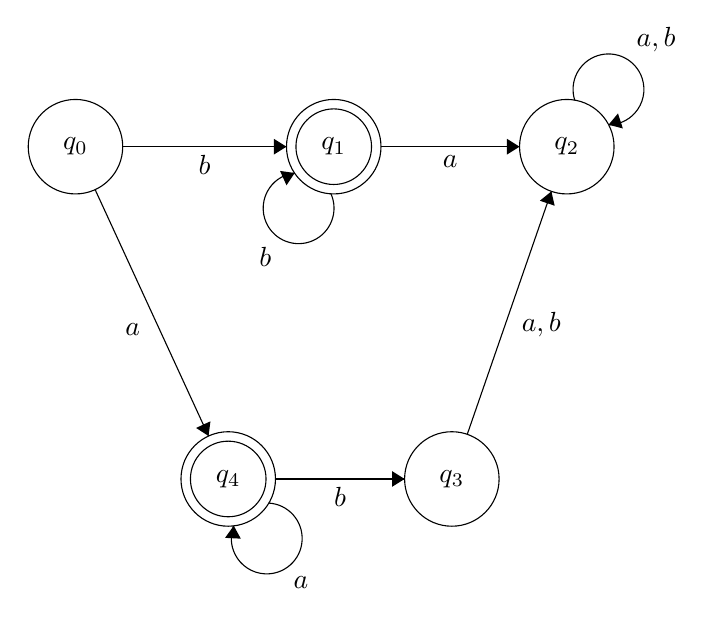
\begin{tikzpicture}[scale=0.2]
\tikzstyle{every node}+=[inner sep=0pt]
\draw [black] (29.3,-21.7) circle (3);
\draw (29.3,-21.7) node {$q_1$};
\draw [black] (29.3,-21.7) circle (2.4);
\draw [black] (44.1,-21.7) circle (3);
\draw (44.1,-21.7) node {$q_2$};
\draw [black] (36.8,-42.8) circle (3);
\draw (36.8,-42.8) node {$q_3$};
\draw [black] (22.6,-42.8) circle (3);
\draw (22.6,-42.8) node {$q_4$};
\draw [black] (22.6,-42.8) circle (2.4);
\draw [black] (12.9,-21.7) circle (3);
\draw (12.9,-21.7) node {$q_0$};
\draw [black] (15.9,-21.7) -- (26.3,-21.7);
\fill [black] (26.3,-21.7) -- (25.5,-21.2) -- (25.5,-22.2);
\draw (21.1,-22.2) node [below] {$b$};
\draw [black] (14.15,-24.43) -- (21.35,-40.07);
\fill [black] (21.35,-40.07) -- (21.47,-39.14) -- (20.56,-39.56);
\draw (17.03,-33.28) node [left] {$a$};
\draw [black] (25.166,-44.331) arc (86.90524:-201.09476:2.25);
\draw (27.21,-48.97) node [below] {$a$};
\fill [black] (22.95,-45.77) -- (22.4,-46.54) -- (23.4,-46.59);
\draw [black] (25.6,-42.8) -- (33.8,-42.8);
\fill [black] (33.8,-42.8) -- (33,-42.3) -- (33,-43.3);
\draw (29.7,-43.3) node [below] {$b$};
\draw [black] (29.119,-24.683) arc (24.25512:-263.74488:2.25);
\draw (24.95,-28.06) node [below] {$b$};
\fill [black] (26.82,-23.37) -- (25.89,-23.24) -- (26.3,-24.15);
\draw [black] (32.3,-21.7) -- (41.1,-21.7);
\fill [black] (41.1,-21.7) -- (40.3,-21.2) -- (40.3,-22.2);
\draw (36.7,-22.2) node [below] {$a$};
\draw [black] (44.607,-18.755) arc (197.97263:-90.02737:2.25);
\draw (49.77,-15.74) node [above] {$a,b$};
\fill [black] (46.75,-20.31) -- (47.66,-20.54) -- (47.35,-19.59);
\draw [black] (37.78,-39.96) -- (43.12,-24.54);
\fill [black] (43.12,-24.54) -- (42.39,-25.13) -- (43.33,-25.45);
\draw (41.21,-32.99) node [right] {$a,b$};
\end{tikzpicture}
\end{center}

\subsection*{b.}
$q_0$ is initial state. $\newline$

\begin{center}
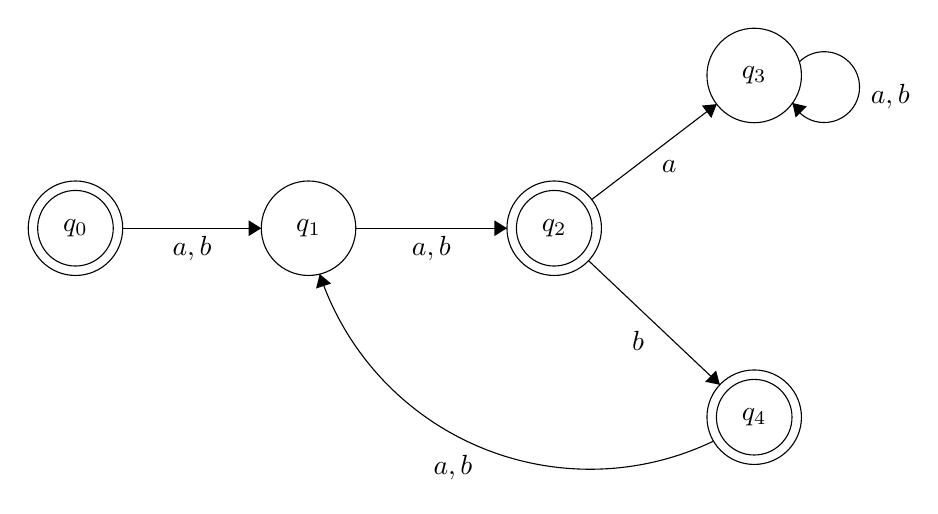
\begin{tikzpicture}[scale=0.2]
\tikzstyle{every node}+=[inner sep=0pt]
\draw [black] (11.2,-21.7) circle (3);
\draw (11.2,-21.7) node {$q_0$};
\draw [black] (11.2,-21.7) circle (2.4);
\draw [black] (26,-21.7) circle (3);
\draw (26,-21.7) node {$q_1$};
\draw [black] (41.6,-21.7) circle (3);
\draw (41.6,-21.7) node {$q_2$};
\draw [black] (41.6,-21.7) circle (2.4);
\draw [black] (54.3,-12) circle (3);
\draw (54.3,-12) node {$q_3$};
\draw [black] (54.3,-33.7) circle (3);
\draw (54.3,-33.7) node {$q_4$};
\draw [black] (54.3,-33.7) circle (2.4);
\draw [black] (14.2,-21.7) -- (23,-21.7);
\fill [black] (23,-21.7) -- (22.2,-21.2) -- (22.2,-22.2);
\draw (18.6,-22.2) node [below] {$a,b$};
\draw [black] (29,-21.7) -- (38.6,-21.7);
\fill [black] (38.6,-21.7) -- (37.8,-21.2) -- (37.8,-22.2);
\draw (33.8,-22.2) node [below] {$a,b$};
\draw [black] (43.98,-19.88) -- (51.92,-13.82);
\fill [black] (51.92,-13.82) -- (50.98,-13.91) -- (51.58,-14.7);
\draw (48.9,-17.35) node [below] {$a$};
\draw [black] (57.161,-11.136) arc (134.53768:-153.46232:2.25);
\draw (61.67,-13.34) node [right] {$a,b$};
\fill [black] (56.73,-13.75) -- (56.93,-14.67) -- (57.64,-13.96);
\draw [black] (43.78,-23.76) -- (52.12,-31.64);
\fill [black] (52.12,-31.64) -- (51.88,-30.73) -- (51.19,-31.45);
\draw (46.93,-28.18) node [below] {$b$};
\draw [black] (51.716,-35.218) arc (-64.32048:-161.63616:18.092);
\fill [black] (26.71,-24.61) -- (26.48,-25.53) -- (27.43,-25.21);
\draw (35.17,-36.09) node [below] {$a,b$};
\end{tikzpicture}
\end{center}

\subsection*{c.}

$q_0$ is initial state. $\newline$

\begin{center}
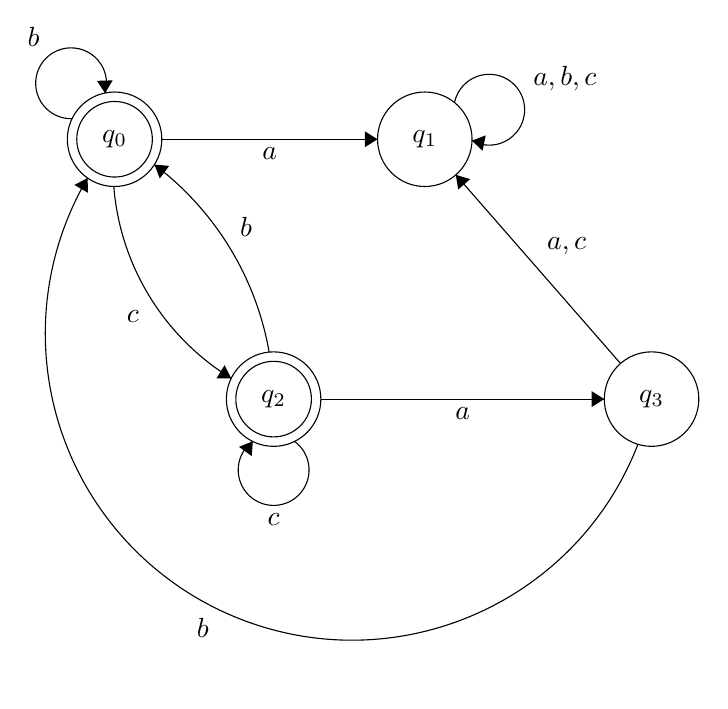
\begin{tikzpicture}[scale=0.2]
\tikzstyle{every node}+=[inner sep=0pt]
\draw [black] (14,-22.2) circle (3);
\draw (14,-22.2) node {$q_0$};
\draw [black] (14,-22.2) circle (2.4);
\draw [black] (33.7,-22.2) circle (3);
\draw (33.7,-22.2) node {$q_1$};
\draw [black] (48.1,-38.7) circle (3);
\draw (48.1,-38.7) node {$q_3$};
\draw [black] (24.1,-38.7) circle (3);
\draw (24.1,-38.7) node {$q_2$};
\draw [black] (24.1,-38.7) circle (2.4);
\draw [black] (11.312,-20.894) arc (271.81301:-16.18699:2.25);
\draw (8.86,-16.37) node [above] {$b$};
\fill [black] (13.4,-19.27) -- (13.88,-18.46) -- (12.88,-18.49);
\draw [black] (17,-22.2) -- (30.7,-22.2);
\fill [black] (30.7,-22.2) -- (29.9,-21.7) -- (29.9,-22.7);
\draw (23.85,-22.7) node [below] {$a$};
\draw [black] (35.585,-19.881) arc (168.62356:-119.37644:2.25);
\draw (40.56,-18.37) node [right] {$a,b,c$};
\fill [black] (36.69,-22.29) -- (37.37,-22.93) -- (37.57,-21.95);
\draw [black] (21.411,-37.381) arc (-121.57815:-175.47849:15.763);
\fill [black] (21.41,-37.38) -- (20.99,-36.54) -- (20.47,-37.39);
\draw (15.58,-33.46) node [left] {$c$};
\draw [black] (16.528,-23.81) arc (52.98919:9.95418:19.03);
\fill [black] (16.53,-23.81) -- (16.87,-24.69) -- (17.47,-23.89);
\draw (21.94,-27.79) node [right] {$b$};
\draw [black] (27.1,-38.7) -- (45.1,-38.7);
\fill [black] (45.1,-38.7) -- (44.3,-38.2) -- (44.3,-39.2);
\draw (36.1,-39.2) node [below] {$a$};
\draw [black] (25.423,-41.38) arc (54:-234:2.25);
\draw (24.1,-45.95) node [below] {$c$};
\fill [black] (22.78,-41.38) -- (21.9,-41.73) -- (22.71,-42.32);
\draw [black] (46.13,-36.44) -- (35.67,-24.46);
\fill [black] (35.67,-24.46) -- (35.82,-25.39) -- (36.58,-24.73);
\draw (41.44,-29) node [right] {$a,c$};
\draw [black] (47.235,-41.569) arc (-21.19166:-210.45032:19.476);
\fill [black] (12.29,-24.66) -- (11.45,-25.1) -- (12.31,-25.6);
\draw (19.61,-52.57) node [below] {$b$};
\end{tikzpicture}
\end{center}

\section*{Answer 3}

\begin{center}
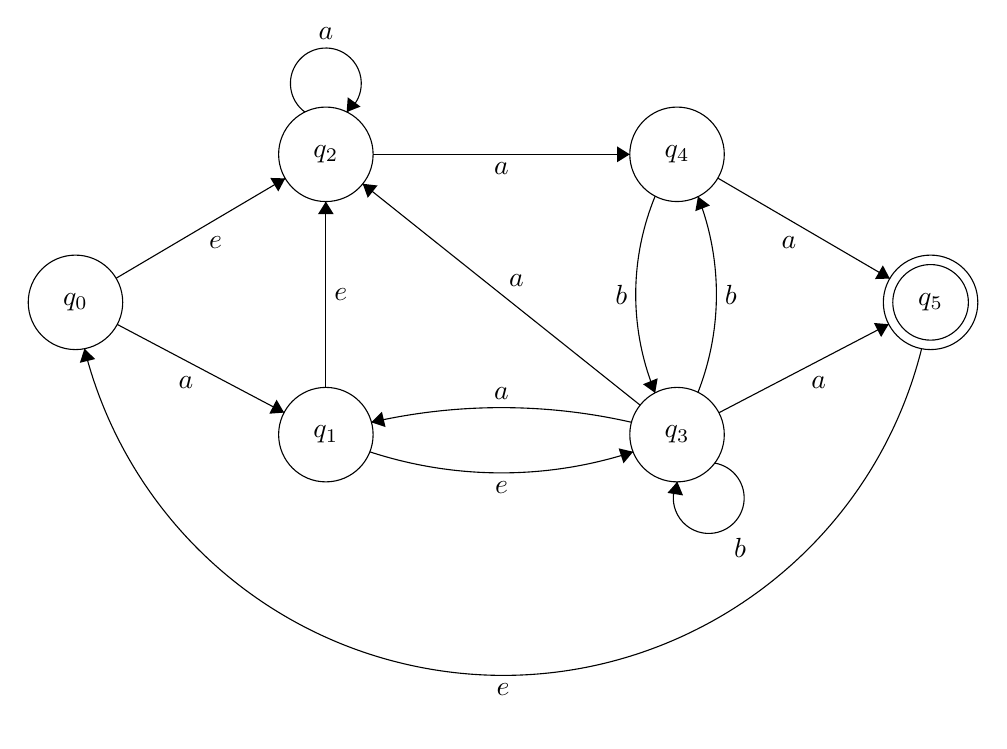
\begin{tikzpicture}[scale=0.2]
\tikzstyle{every node}+=[inner sep=0pt]
\draw [black] (13.3,-24.8) circle (3);
\draw (13.3,-24.8) node {$q_0$};
\draw [black] (29.2,-33.2) circle (3);
\draw (29.2,-33.2) node {$q_1$};
\draw [black] (29.2,-15.4) circle (3);
\draw (29.2,-15.4) node {$q_2$};
\draw [black] (51.5,-33.2) circle (3);
\draw (51.5,-33.2) node {$q_3$};
\draw [black] (51.5,-15.4) circle (3);
\draw (51.5,-15.4) node {$q_4$};
\draw [black] (67.6,-24.8) circle (3);
\draw (67.6,-24.8) node {$q_5$};
\draw [black] (67.6,-24.8) circle (2.4);
\draw [black] (15.88,-23.27) -- (26.62,-16.93);
\fill [black] (26.62,-16.93) -- (25.67,-16.9) -- (26.18,-17.76);
\draw (22.19,-20.6) node [below] {$e$};
\draw [black] (15.95,-26.2) -- (26.55,-31.8);
\fill [black] (26.55,-31.8) -- (26.07,-30.98) -- (25.61,-31.87);
\draw (20.31,-29.5) node [below] {$a$};
\draw [black] (48.708,-34.293) arc (-71.83165:-108.16835:26.804);
\fill [black] (48.71,-34.29) -- (47.79,-34.07) -- (48.1,-35.02);
\draw (40.35,-36.13) node [below] {$e$};
\draw [black] (53.881,-35.005) arc (80.56505:-207.43495:2.25);
\draw (55.51,-39.74) node [below] {$b$};
\fill [black] (51.52,-36.19) -- (50.89,-36.9) -- (51.88,-37.06);
\draw [black] (52.83,-18.085) arc (21.33334:-21.33334:17.085);
\fill [black] (52.83,-18.08) -- (52.66,-19.01) -- (53.59,-18.65);
\draw (54.5,-24.3) node [right] {$b$};
\draw [black] (49.16,-31.33) -- (31.54,-17.27);
\fill [black] (31.54,-17.27) -- (31.86,-18.16) -- (32.48,-17.38);
\draw (41.3,-23.81) node [above] {$a$};
\draw [black] (29.2,-30.2) -- (29.2,-18.4);
\fill [black] (29.2,-18.4) -- (28.7,-19.2) -- (29.7,-19.2);
\draw (29.7,-24.3) node [right] {$e$};
\draw [black] (32.2,-15.4) -- (48.5,-15.4);
\fill [black] (48.5,-15.4) -- (47.7,-14.9) -- (47.7,-15.9);
\draw (40.35,-15.9) node [below] {$a$};
\draw [black] (27.877,-12.72) arc (234:-54:2.25);
\draw (29.2,-8.15) node [above] {$a$};
\fill [black] (30.52,-12.72) -- (31.4,-12.37) -- (30.59,-11.78);
\draw [black] (32.095,-32.415) arc (102.85472:77.14528:37.106);
\fill [black] (32.09,-32.42) -- (32.99,-32.72) -- (32.76,-31.75);
\draw (40.35,-30.99) node [above] {$a$};
\draw [black] (54.16,-31.81) -- (64.94,-26.19);
\fill [black] (64.94,-26.19) -- (64,-26.11) -- (64.46,-27);
\draw (60.49,-29.5) node [below] {$a$};
\draw [black] (54.09,-16.91) -- (65.01,-23.29);
\fill [black] (65.01,-23.29) -- (64.57,-22.45) -- (64.07,-23.32);
\draw (58.61,-20.6) node [below] {$a$};
\draw [black] (50.111,-30.546) arc (-157.61711:-202.38289:16.402);
\fill [black] (50.11,-30.55) -- (50.27,-29.62) -- (49.34,-30);
\draw (48.38,-24.3) node [left] {$b$};
\draw [black] (67.031,-27.744) arc (-14.07909:-165.92091:27.404);
\fill [black] (13.87,-27.74) -- (13.58,-28.64) -- (14.55,-28.4);
\draw (40.45,-48.98) node [below] {$e$};
\end{tikzpicture}
\end{center}

\subsection*{a.}
It is clear to see that a word must end with $a$. Since $w$ does not end with $a$, it is not in the language. $\newline$

\subsection*{b.}
We can find a path from our initial state to final state. The path is: $\newline$

\begin{align*}
(q_0,a,q_1), (q_1,e,q_3), (q_3,b,q_3), (q_3,a,q_1), (q_1,e,q_3), (q_3,b,q_3),
(q_3,a,q_5)
\end{align*}

\section*{Answer 4}

\subsection*{a.}

\begin{center}
\begin{tikzpicture}[scale=0.2]
\tikzstyle{every node}+=[inner sep=0pt]
\draw [black] (19.1,-28.5) circle (3);
\draw (19.1,-28.5) node {$q_0$};
\draw [black] (33.6,-28.5) circle (3);
\draw (33.6,-28.5) node {$q_1$};
\draw [black] (47.7,-16.8) circle (3);
\draw (47.7,-16.8) node {$q_2$};
\draw [black] (47.7,-39.4) circle (3);
\draw (47.7,-39.4) node {$q_3$};
\draw [black] (4.7,-28) circle (3);
\draw (4.7,-28) node {$q_{init}$};
\draw [black] (66.5,-28) circle (3);
\draw (66.5,-28) node {$q_{fin}$};
\draw [black] (66.5,-28) circle (2.4);
\draw [black] (22.1,-28.5) -- (30.6,-28.5);
\fill [black] (30.6,-28.5) -- (29.8,-28) -- (29.8,-29);
\draw (26.35,-29) node [below] {$b$};
\draw [black] (46.436,-19.517) arc (-29.65525:-70.97384:18.291);
\fill [black] (46.44,-19.52) -- (45.61,-19.96) -- (46.47,-20.46);
\draw (43.17,-25.04) node [below] {$a$};
\draw [black] (36.546,-29.042) arc (74.39448:30.19391:16.607);
\fill [black] (46.43,-36.69) -- (46.46,-35.74) -- (45.6,-36.25);
\draw (43.19,-31.4) node [above] {$e$};
\draw [black] (19.993,-25.639) arc (158.10678:66.39126:18.869);
\fill [black] (19.99,-25.64) -- (20.76,-25.08) -- (19.83,-24.71);
\draw (29.45,-14.7) node [above] {$a$};
\draw [black] (34.729,-25.725) arc (152.70568:106.66523:16.673);
\fill [black] (34.73,-25.72) -- (35.54,-25.24) -- (34.65,-24.78);
\draw (37.89,-20.05) node [above] {$b$};
\draw [black] (48.14,-13.844) arc (199.26738:-88.73262:2.25);
\draw (52.55,-10.75) node [above] {$b$};
\fill [black] (50.31,-15.35) -- (51.23,-15.56) -- (50.9,-14.62);
\draw [black] (47.7,-19.8) -- (47.7,-36.4);
\fill [black] (47.7,-36.4) -- (48.2,-35.6) -- (47.2,-35.6);
\draw (47.2,-28.1) node [left] {$b$};
\draw [black] (44.805,-38.626) arc (-109.37047:-146.04114:19.54);
\fill [black] (35.08,-31.11) -- (35.11,-32.05) -- (35.94,-31.49);
\draw (38.33,-36.15) node [below] {$b$};
\draw [black] (49.023,-42.08) arc (54:-234:2.25);
\draw (47.7,-46.65) node [below] {$a$};
\fill [black] (46.38,-42.08) -- (45.5,-42.43) -- (46.31,-43.02);
\draw [black] (7.7,-28.1) -- (16.1,-28.4);
\fill [black] (16.1,-28.4) -- (15.32,-27.87) -- (15.28,-28.87);
\draw (11.88,-28.78) node [below] {$e$};
\draw [black] (50.28,-18.34) -- (63.92,-26.46);
\fill [black] (63.92,-26.46) -- (63.49,-25.63) -- (62.98,-26.48);
\draw (56.16,-22.9) node [below] {$e$};
\draw [black] (50.27,-37.84) -- (63.93,-29.56);
\fill [black] (63.93,-29.56) -- (62.99,-29.54) -- (63.51,-30.4);
\draw (58.04,-34.2) node [below] {$e$};
\end{tikzpicture}
\end{center}

\subsection*{b.}
First, delete $q_0$. $\newline$

\begin{center}
\begin{tikzpicture}[scale=0.2]
\tikzstyle{every node}+=[inner sep=0pt]
\draw [black] (26,-28) circle (3);
\draw (26,-28) node {$q_1$};
\draw [black] (47.7,-16.8) circle (3);
\draw (47.7,-16.8) node {$q_2$};
\draw [black] (47.7,-39.4) circle (3);
\draw (47.7,-39.4) node {$q_3$};
\draw [black] (7.6,-28) circle (3);
\draw (7.6,-28) node {$q_{init}$};
\draw [black] (66.5,-28) circle (3);
\draw (66.5,-28) node {$q_{fin}$};
\draw [black] (66.5,-28) circle (2.4);
\draw [black] (45.668,-19.006) arc (-45.37176:-80.0291:31.535);
\fill [black] (45.67,-19.01) -- (44.75,-19.21) -- (45.45,-19.92);
\draw (38.92,-25.09) node [below] {$a$};
\draw [black] (28.979,-28.348) arc (80.5019:44.06811:30.253);
\fill [black] (45.72,-37.14) -- (45.53,-36.22) -- (44.81,-36.92);
\draw (38.99,-30.9) node [above] {$e$};
\draw [black] (27.943,-25.716) arc (136.59738:98.00176:28.552);
\fill [black] (27.94,-25.72) -- (28.86,-25.48) -- (28.13,-24.79);
\draw (32.85,-19.45) node [above] {$b+\mbox{ }ab$};
\draw [black] (48.14,-13.844) arc (199.26738:-88.73262:2.25);
\draw (52.55,-10.75) node [above] {$b$};
\fill [black] (50.31,-15.35) -- (51.23,-15.56) -- (50.9,-14.62);
\draw [black] (47.7,-19.8) -- (47.7,-36.4);
\fill [black] (47.7,-36.4) -- (48.2,-35.6) -- (47.2,-35.6);
\draw (47.2,-28.1) node [left] {$b$};
\draw [black] (44.748,-38.869) arc (-102.58717:-132.84282:36.004);
\fill [black] (28.11,-30.13) -- (28.36,-31.04) -- (29.04,-30.31);
\draw (34.86,-36.11) node [below] {$b$};
\draw [black] (49.023,-42.08) arc (54:-234:2.25);
\draw (47.7,-46.65) node [below] {$a$};
\fill [black] (46.38,-42.08) -- (45.5,-42.43) -- (46.31,-43.02);
\draw [black] (50.28,-18.34) -- (63.92,-26.46);
\fill [black] (63.92,-26.46) -- (63.49,-25.63) -- (62.98,-26.48);
\draw (56.16,-22.9) node [below] {$e$};
\draw [black] (50.27,-37.84) -- (63.93,-29.56);
\fill [black] (63.93,-29.56) -- (62.99,-29.54) -- (63.51,-30.4);
\draw (58.04,-34.2) node [below] {$e$};
\draw [black] (10.6,-28) -- (23,-28);
\fill [black] (23,-28) -- (22.2,-27.5) -- (22.2,-28.5);
\end{tikzpicture}
\end{center}

Then, we delete $q_3$. $\newline$

\begin{center}
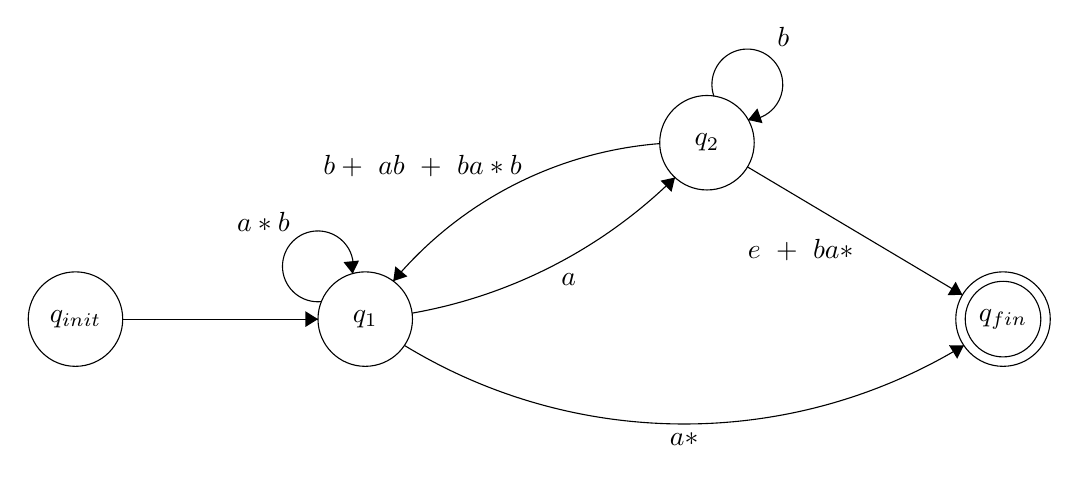
\begin{tikzpicture}[scale=0.2]
\tikzstyle{every node}+=[inner sep=0pt]
\draw [black] (26,-28) circle (3);
\draw (26,-28) node {$q_1$};
\draw [black] (47.7,-16.8) circle (3);
\draw (47.7,-16.8) node {$q_2$};
\draw [black] (7.6,-28) circle (3);
\draw (7.6,-28) node {$q_{init}$};
\draw [black] (66.5,-28) circle (3);
\draw (66.5,-28) node {$q_{fin}$};
\draw [black] (66.5,-28) circle (2.4);
\draw [black] (45.668,-19.006) arc (-45.37176:-80.0291:31.535);
\fill [black] (45.67,-19.01) -- (44.75,-19.21) -- (45.45,-19.92);
\draw (38.92,-25.09) node [below] {$a$};
\draw [black] (27.78,-25.588) arc (140.081:94.51815:24.59);
\fill [black] (27.78,-25.59) -- (28.68,-25.29) -- (27.91,-24.65);
\draw (29.64,-19) node [above] {$b+\mbox{ }ab\mbox{ }+\mbox{ }ba*b$};
\draw [black] (48.14,-13.844) arc (199.26738:-88.73262:2.25);
\draw (52.55,-10.75) node [above] {$b$};
\fill [black] (50.31,-15.35) -- (51.23,-15.56) -- (50.9,-14.62);
\draw [black] (50.28,-18.34) -- (63.92,-26.46);
\fill [black] (63.92,-26.46) -- (63.49,-25.63) -- (62.98,-26.48);
\draw (53.65,-22.9) node [below] {$e\mbox{ }+\mbox{ }ba*$};
\draw [black] (10.6,-28) -- (23,-28);
\fill [black] (23,-28) -- (22.2,-27.5) -- (22.2,-28.5);
\draw [black] (23.226,-26.888) arc (275.89215:-12.10785:2.25);
\draw (19.54,-22.49) node [above] {$a*b$};
\fill [black] (25.2,-25.12) -- (25.61,-24.28) -- (24.62,-24.38);
\draw [black] (64.011,-29.673) arc (-58.62001:-121.37999:34.109);
\fill [black] (64.01,-29.67) -- (63.07,-29.66) -- (63.59,-30.52);
\draw (46.25,-35.16) node [below] {$a*$};
\end{tikzpicture}
\end{center}

Then, we delete $q_1$. $\newline$

\begin{center}
\begin{tikzpicture}[scale=0.2]
\tikzstyle{every node}+=[inner sep=0pt]
\draw [black] (6.6,-25.7) circle (3);
\draw (6.6,-25.7) node {$q_{init}$};
\draw [black] (64.7,-25.7) circle (3);
\draw (64.7,-25.7) node {$q_{fin}$};
\draw [black] (64.7,-25.7) circle (2.4);
\draw [black] (34.2,-25.7) circle (3);
\draw (34.2,-25.7) node {$q_2$};
\draw [black] (9.6,-25.7) -- (31.2,-25.7);
\fill [black] (31.2,-25.7) -- (30.4,-25.2) -- (30.4,-26.2);
\draw [black] (32.877,-23.02) arc (234:-54:2.25);
\draw (34.2,-18.45) node [above] {$b+((b+ab+ba*b)(a*b)*a)$};
\fill [black] (35.52,-23.02) -- (36.4,-22.67) -- (35.59,-22.08);
\draw [black] (65.034,-28.677) arc (0.89539:-180.89539:15.586);
\fill [black] (65.03,-28.68) -- (64.55,-29.48) -- (65.55,-29.47);
\draw (49.45,-45.01) node [below] {$(e+ba*)+(b+ab+ba*b)(a*b)a*$};
\draw [black] (8.025,-23.062) arc (148.95433:31.04567:32.243);
\fill [black] (63.27,-23.06) -- (63.29,-22.12) -- (62.43,-22.63);
\draw (35.65,-6.95) node [above] {$a*ba*$};
\end{tikzpicture}
\end{center}

Finally, we delete $q_2$ $\newline$

\begin{center}
\begin{tikzpicture}[scale=0.2]
\tikzstyle{every node}+=[inner sep=0pt]
\draw [black] (9.4,-16.2) circle (3);
\draw (9.4,-16.2) node {$q_{init}$};
\draw [black] (69.1,-16.2) circle (3);
\draw (69.1,-16.2) node {$q_{fin}$};
\draw [black] (69.1,-16.2) circle (2.4);
\draw [black] (69.139,-19.198) arc (-2.13133:-177.86867:29.91);
\fill [black] (69.14,-19.2) -- (68.61,-19.98) -- (69.61,-20.02);
\draw (39.25,-48.5) node [below] {$(a*ba*)+((ba((b+ab+ba*b)a*b)*a))*((e+ba*)+(b+ab+ba*b)(a*b)a*))$};
\end{tikzpicture}
\end{center}

\section*{Answer 5}

\subsection*{a.}

${q_0}$ is initial.

\begin{center}
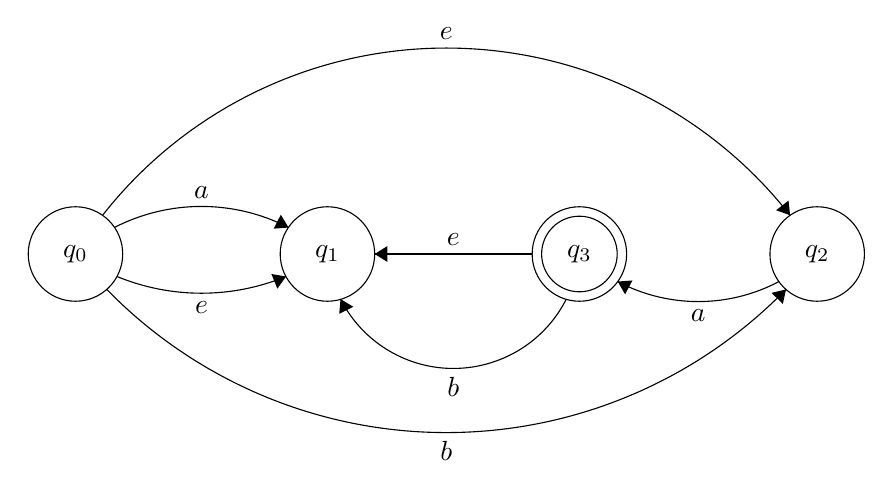
\begin{tikzpicture}[scale=0.2]
\tikzstyle{every node}+=[inner sep=0pt]
\draw [black] (12.6,-20.5) circle (3);
\draw (12.6,-20.5) node {$q_0$};
\draw [black] (28.6,-20.5) circle (3);
\draw (28.6,-20.5) node {$q_1$};
\draw [black] (59.7,-20.5) circle (3);
\draw (59.7,-20.5) node {$q_2$};
\draw [black] (44.6,-20.5) circle (3);
\draw (44.6,-20.5) node {$q_3$};
\draw [black] (44.6,-20.5) circle (2.4);
\draw [black] (15.073,-18.815) arc (117.16927:62.83073:12.104);
\fill [black] (26.13,-18.82) -- (25.64,-18) -- (25.19,-18.89);
\draw (20.6,-16.98) node [above] {$a$};
\draw [black] (25.968,-21.928) arc (-67.60597:-112.39403:14.091);
\fill [black] (25.97,-21.93) -- (25.04,-21.77) -- (25.42,-22.7);
\draw (20.6,-23.49) node [below] {$e$};
\draw [black] (57.716,-22.748) arc (-44.28054:-135.71946:30.123);
\fill [black] (57.72,-22.75) -- (56.8,-22.97) -- (57.52,-23.67);
\draw (36.15,-32.34) node [below] {$b$};
\draw [black] (14.32,-18.044) arc (141.89291:38.10709:27.743);
\fill [black] (57.98,-18.04) -- (57.88,-17.11) -- (57.09,-17.72);
\draw (36.15,-6.92) node [above] {$e$};
\draw [black] (57.274,-22.248) arc (-62.08277:-117.91723:10.943);
\fill [black] (47.03,-22.25) -- (47.5,-23.06) -- (47.97,-22.18);
\draw (52.15,-24.02) node [below] {$a$};
\draw [black] (43.768,-23.364) arc (-26.8909:-153.1091:8.037);
\fill [black] (29.43,-23.36) -- (29.35,-24.3) -- (30.24,-23.85);
\draw (36.6,-28.27) node [below] {$b$};
\draw [black] (41.6,-20.5) -- (31.6,-20.5);
\fill [black] (31.6,-20.5) -- (32.4,-21) -- (32.4,-20);
\draw (36.6,-20) node [above] {$e$};
\end{tikzpicture}
\end{center}

Table is:

\begin{tabular}{l|l|l|l}
My names & States      & a        & b        \\ \hline
A        & emptyset    & emptyset & emptyset \\
\hline
B        & q0          & q1       & q2       \\ \hline
C        & q1          & emptyset & emptyset \\ \hline
D        & q2          & q3       & emptyset \\ \hline
E        & q3          & emptset  & q1       \\ \hline
F        & q0,q1       & q1       & q2       \\ \hline
G        & q0,q2       & q1,q3    & q2       \\ \hline
H        & q0,q3       & q1       & q1,q2    \\ \hline
I        & q1,q2       & q3       & emptyset \\ \hline
J        & q1,q3       & emptyset & q1       \\ \hline
K        & q2,q3       & q3       & q1       \\ \hline
L        & q0,q1,q2    & q1,q3    & q2       \\ \hline
M        & q0,q1,q3    & q1       & q1,q2    \\ \hline
N        & q0,q2,q3    & q1,q3    & q1,q2    \\ \hline
O        & q1,q2,q3    & q3       & q1       \\ \hline
P        & q0,q1,q2,q3 & q1,q3    & q1,q2   
\end{tabular}
\\
Lets start with N, because it has one of the most states. Table for N is in below: \\

\begin{tabular}{l|l|l|l}
Name & a & b \\ \hline
N    & J & I \\ \hline
J    & A & C \\ \hline
I    & E & A \\ \hline
A    & A & A \\ \hline
E    & A & C \\ \hline
C    & A & A \\
\end{tabular}
\\
And the diagram is: \\

\begin{center}
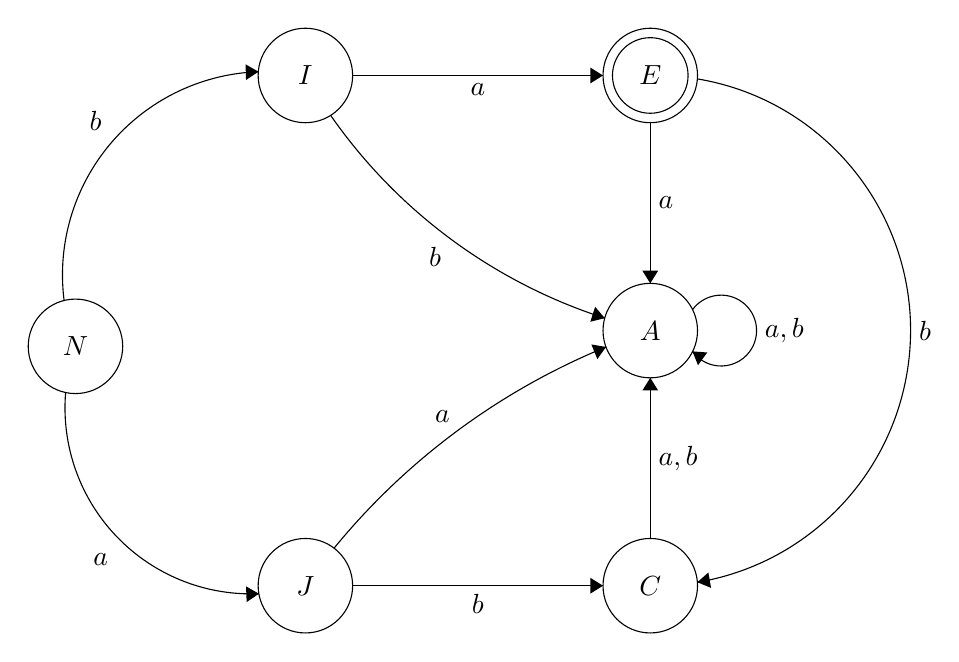
\begin{tikzpicture}[scale=0.2]
\tikzstyle{every node}+=[inner sep=0pt]
\draw [black] (7.8,-26.5) circle (3);
\draw (7.8,-26.5) node {$N$};
\draw [black] (22.4,-41.7) circle (3);
\draw (22.4,-41.7) node {$J$};
\draw [black] (22.4,-9.3) circle (3);
\draw (22.4,-9.3) node {$I$};
\draw [black] (44.3,-25.5) circle (3);
\draw (44.3,-25.5) node {$A$};
\draw [black] (44.3,-41.7) circle (3);
\draw (44.3,-41.7) node {$C$};
\draw [black] (44.3,-9.3) circle (3);
\draw (44.3,-9.3) node {$E$};
\draw [black] (44.3,-9.3) circle (2.4);
\draw [black] (19.451,-42.207) arc (-87.52704:-184.77986:11.808);
\fill [black] (19.45,-42.21) -- (18.63,-41.74) -- (18.67,-42.74);
\draw (9.9,-40.06) node [left] {$a$};
\draw [black] (7.079,-23.595) arc (-172.72783:-267.92385:12.908);
\fill [black] (19.42,-9.06) -- (18.6,-8.59) -- (18.63,-9.59);
\draw (9.49,-12.17) node [left] {$b$};
\draw [black] (24.22,-39.316) arc (140.68346:112.29913:43.803);
\fill [black] (41.49,-26.54) -- (40.56,-26.38) -- (40.94,-27.31);
\draw (31.11,-31.36) node [above] {$a$};
\draw [black] (25.4,-41.7) -- (41.3,-41.7);
\fill [black] (41.3,-41.7) -- (40.5,-41.2) -- (40.5,-42.2);
\draw (33.35,-42.2) node [below] {$b$};
\draw [black] (25.4,-9.3) -- (41.3,-9.3);
\fill [black] (41.3,-9.3) -- (40.5,-8.8) -- (40.5,-9.8);
\draw (33.35,-9.8) node [below] {$a$};
\draw [black] (41.407,-24.708) arc (-107.84246:-145.14013:33.85);
\fill [black] (41.41,-24.71) -- (40.8,-23.99) -- (40.49,-24.94);
\draw (30.64,-20.2) node [below] {$b$};
\draw [black] (46.98,-24.177) arc (144:-144:2.25);
\draw (51.55,-25.5) node [right] {$a,b$};
\fill [black] (46.98,-26.82) -- (47.33,-27.7) -- (47.92,-26.89);
\draw [black] (44.3,-12.3) -- (44.3,-22.5);
\fill [black] (44.3,-22.5) -- (44.8,-21.7) -- (43.8,-21.7);
\draw (44.8,-17.4) node [right] {$a$};
\draw [black] (47.288,-9.517) arc (80.53989:-80.53989:16.203);
\fill [black] (47.29,-41.48) -- (48.16,-41.84) -- (47.99,-40.86);
\draw (61.33,-25.5) node [right] {$b$};
\draw [black] (44.3,-38.7) -- (44.3,-28.5);
\fill [black] (44.3,-28.5) -- (43.8,-29.3) -- (44.8,-29.3);
\draw (44.8,-33.6) node [right] {$a,b$};
\end{tikzpicture}
\end{center}

\subsection*{b.}

\section*{Answer 6}

Let ${L_1}$ and ${L_2}$ denote two reguar languages. Then, the following is also regular:

\begin{align*}
{L_1}' = \{ x \in \Sigma^* | x \notin L_1 \}
\end{align*}

Meaning that, ${L_1}'$ is compliment of ${L_1}$. We can also use union property of language to obtain:

\begin{align*}
L_1 \setminus L_2 = L_1 \cap L_2' = (L_1' \cup L_2)'
\end{align*}

Now, let L1 is the language of the left figure and L2 is the language of the right figure.
\begin{center}
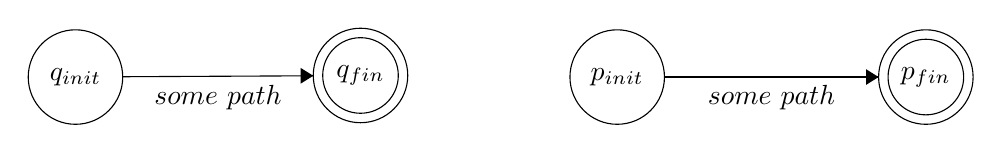
\begin{tikzpicture}[scale=0.2]
\tikzstyle{every node}+=[inner sep=0pt]
\draw [black] (9.4,-20.1) circle (3);
\draw (9.4,-20.1) node {$q_{init}$};
\draw [black] (27.5,-20) circle (3);
\draw (27.5,-20) node {$q_{fin}$};
\draw [black] (27.5,-20) circle (2.4);
\draw [black] (43.8,-20.1) circle (3);
\draw (43.8,-20.1) node {$p_{init}$};
\draw [black] (63.4,-20.1) circle (3);
\draw (63.4,-20.1) node {$p_{fin}$};
\draw [black] (63.4,-20.1) circle (2.4);
\draw [black] (12.4,-20.08) -- (24.5,-20.02);
\fill [black] (24.5,-20.02) -- (23.7,-19.52) -- (23.7,-20.52);
\draw (18.45,-20.58) node [below] {$some\mbox{ }path$};
\draw [black] (46.8,-20.1) -- (60.4,-20.1);
\fill [black] (60.4,-20.1) -- (59.6,-19.6) -- (59.6,-20.6);
\draw (53.6,-20.6) node [below] {$some\mbox{ }path$};
\end{tikzpicture}
\end{center}

By complementing ${L_1}$, we obtain: 

\begin{center}
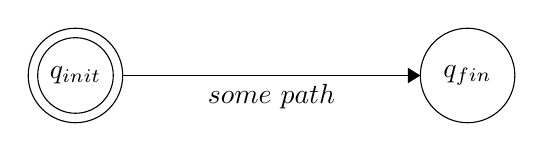
\begin{tikzpicture}[scale=0.2]
\tikzstyle{every node}+=[inner sep=0pt]
\draw [black] (16.8,-19.4) circle (3);
\draw (16.8,-19.4) node {$q_{init}$};
\draw [black] (16.8,-19.4) circle (2.4);
\draw [black] (41.7,-19.4) circle (3);
\draw (41.7,-19.4) node {$q_{fin}$};
\draw [black] (19.8,-19.4) -- (38.7,-19.4);
\fill [black] (38.7,-19.4) -- (37.9,-18.9) -- (37.9,-19.9);
\draw (29.25,-19.9) node [below] {$some\mbox{ }path$};
\end{tikzpicture}
\end{center}

Using union property, we obtain:

\begin{center}
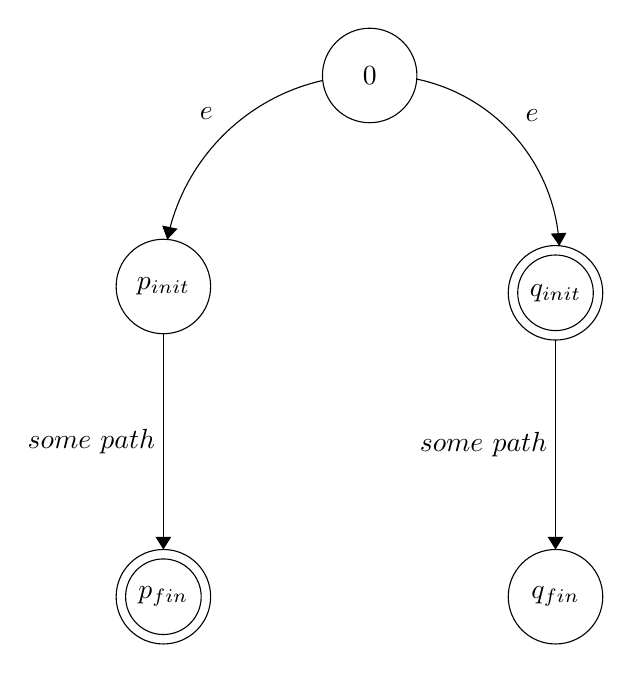
\begin{tikzpicture}[scale=0.2]
\tikzstyle{every node}+=[inner sep=0pt]
\draw [black] (51,-21.2) circle (3);
\draw (51,-21.2) node {$q_{init}$};
\draw [black] (51,-21.2) circle (2.4);
\draw [black] (51,-40.5) circle (3);
\draw (51,-40.5) node {$q_{fin}$};
\draw [black] (26.1,-20.8) circle (3);
\draw (26.1,-20.8) node {$p_{init}$};
\draw [black] (26.1,-40.5) circle (3);
\draw (26.1,-40.5) node {$p_{fin}$};
\draw [black] (26.1,-40.5) circle (2.4);
\draw [black] (39.2,-7.4) circle (3);
\draw (39.2,-7.4) node {$0$};
\draw [black] (51,-24.2) -- (51,-37.5);
\fill [black] (51,-37.5) -- (51.5,-36.7) -- (50.5,-36.7);
\draw (50.5,-30.85) node [left] {$some\mbox{ }path$};
\draw [black] (26.1,-23.8) -- (26.1,-37.5);
\fill [black] (26.1,-37.5) -- (26.6,-36.7) -- (25.6,-36.7);
\draw (25.6,-30.65) node [left] {$some\mbox{ }path$};
\draw [black] (26.349,-17.817) arc (-191.39284:-257.30995:12.982);
\fill [black] (26.35,-17.82) -- (27,-17.13) -- (26.02,-16.93);
\draw (29.27,-9.83) node [left] {$e$};
\draw [black] (42.183,-7.627) arc (78.12335:2.94233:11.422);
\fill [black] (51.24,-18.22) -- (51.7,-17.39) -- (50.7,-17.44);
\draw (49.06,-9.94) node [right] {$e$};
\end{tikzpicture}
\end{center}

And, by complementing the figure above, we can construct the difference operation on regular languages.

\begin{center}
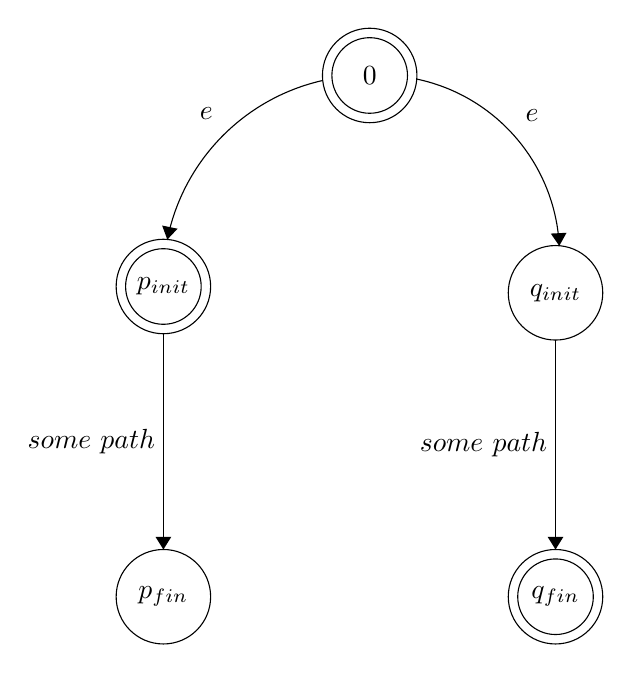
\begin{tikzpicture}[scale=0.2]
\tikzstyle{every node}+=[inner sep=0pt]
\draw [black] (51,-21.2) circle (3);
\draw (51,-21.2) node {$q_{init}$};
\draw [black] (51,-40.5) circle (3);
\draw (51,-40.5) node {$q_{fin}$};
\draw [black] (51,-40.5) circle (2.4);
\draw [black] (26.1,-20.8) circle (3);
\draw (26.1,-20.8) node {$p_{init}$};
\draw [black] (26.1,-20.8) circle (2.4);
\draw [black] (26.1,-40.5) circle (3);
\draw (26.1,-40.5) node {$p_{fin}$};
\draw [black] (39.2,-7.4) circle (3);
\draw (39.2,-7.4) node {$0$};
\draw [black] (39.2,-7.4) circle (2.4);
\draw [black] (51,-24.2) -- (51,-37.5);
\fill [black] (51,-37.5) -- (51.5,-36.7) -- (50.5,-36.7);
\draw (50.5,-30.85) node [left] {$some\mbox{ }path$};
\draw [black] (26.1,-23.8) -- (26.1,-37.5);
\fill [black] (26.1,-37.5) -- (26.6,-36.7) -- (25.6,-36.7);
\draw (25.6,-30.65) node [left] {$some\mbox{ }path$};
\draw [black] (26.349,-17.817) arc (-191.39284:-257.30995:12.982);
\fill [black] (26.35,-17.82) -- (27,-17.13) -- (26.02,-16.93);
\draw (29.27,-9.83) node [left] {$e$};
\draw [black] (42.183,-7.627) arc (78.12335:2.94233:11.422);
\fill [black] (51.24,-18.22) -- (51.7,-17.39) -- (50.7,-17.44);
\draw (49.06,-9.94) node [right] {$e$};
\end{tikzpicture}
\end{center}


\section*{Answer 7}

\subsection*{a.}

If a language $L$ is regular, then there exists a number $n \geq 1$ s.t. every string $uwv$ in $L$ with $|w| \geq n$ can be written in the form $ w = xyz$ s.t. $|y| \geq 1$ and $|xy| \leq n$ and $xy^iz \in L$ for $i \geq 0$.



\end{document}
